\documentclass[11pt,a4paper]{article}
\newcommand{\intestazione}{Dimero di spin --- 3. Dinamica}
% =====================================================================
%  Preambolo comune ai documenti sul dimero (serie "che cosa abbiamo fatto")
%  Incluso con % =====================================================================
%  Preambolo comune ai documenti sul dimero (serie "che cosa abbiamo fatto")
%  Incluso con % =====================================================================
%  Preambolo comune ai documenti sul dimero (serie "che cosa abbiamo fatto")
%  Incluso con \input{preambolo_dimero} subito dopo \documentclass.
% =====================================================================
\usepackage[T1]{fontenc}
\usepackage[utf8]{inputenc}
\usepackage[main=italian,provide=*]{babel}
\usepackage{amsmath,amssymb,mathtools}
\usepackage{graphicx}
\usepackage{booktabs}
\usepackage{colortbl}
\usepackage{xcolor}
\usepackage{geometry}
\usepackage{placeins}
\usepackage{caption}
\usepackage{enumitem}
\usepackage{fancyhdr}
\usepackage{needspace}
\usepackage{tikz}
\usetikzlibrary{arrows.meta,positioning,shapes.geometric,calc,fit,backgrounds}
\usepackage{hyperref}
\hypersetup{colorlinks=true,linkcolor=blu,citecolor=blu,urlcolor=blu}

\geometry{margin=2.5cm}

% --- colori coerenti con quelli delle figure (palette Okabe-Ito)
\definecolor{blu}{HTML}{0072B2}
\definecolor{arancio}{HTML}{E69F00}
\definecolor{verdes}{HTML}{009E73}
\definecolor{rossos}{HTML}{D55E00}
\definecolor{violas}{HTML}{CC79A7}
\definecolor{grigetto}{HTML}{E8E8E8}

\captionsetup{font=small,labelfont=bf,width=0.92\textwidth}

\pagestyle{fancy}
\fancyhf{}
\fancyhead[L]{\small\itshape\intestazione}
\fancyhead[R]{\small\thepage}
\renewcommand{\headrulewidth}{0.3pt}

% --- notazione
\newcommand{\ket}[1]{\lvert #1\rangle}
\newcommand{\bra}[1]{\langle #1 \rvert}
\newcommand{\media}[1]{\langle #1 \rangle}
\newcommand{\vs}[1]{\mathbf{s}_{#1}}

% --- riquadro "in una riga": il messaggio da portare a casa
\newcommand{\messaggio}[1]{%
  \begin{center}
  \begin{minipage}{0.93\textwidth}
  \setlength{\fboxsep}{9pt}%
  \colorbox{grigetto}{\begin{minipage}{\dimexpr\textwidth-2\fboxsep}
  \small\textbf{In una riga.}\enspace #1
  \end{minipage}}
  \end{minipage}
  \end{center}
}

% --- riquadro "come lo sappiamo": la verifica numerica dietro un'affermazione
\newcommand{\verifica}[1]{%
  \begin{center}
  \begin{minipage}{0.93\textwidth}
  \small\textcolor{verdes}{\rule{2.2em}{1.1pt}}\enspace
  \textcolor{verdes}{\textbf{Come lo sappiamo.}}\enspace #1
  \end{minipage}
  \end{center}
  \medskip
}
 subito dopo \documentclass.
% =====================================================================
\usepackage[T1]{fontenc}
\usepackage[utf8]{inputenc}
\usepackage[main=italian,provide=*]{babel}
\usepackage{amsmath,amssymb,mathtools}
\usepackage{graphicx}
\usepackage{booktabs}
\usepackage{colortbl}
\usepackage{xcolor}
\usepackage{geometry}
\usepackage{placeins}
\usepackage{caption}
\usepackage{enumitem}
\usepackage{fancyhdr}
\usepackage{needspace}
\usepackage{tikz}
\usetikzlibrary{arrows.meta,positioning,shapes.geometric,calc,fit,backgrounds}
\usepackage{hyperref}
\hypersetup{colorlinks=true,linkcolor=blu,citecolor=blu,urlcolor=blu}

\geometry{margin=2.5cm}

% --- colori coerenti con quelli delle figure (palette Okabe-Ito)
\definecolor{blu}{HTML}{0072B2}
\definecolor{arancio}{HTML}{E69F00}
\definecolor{verdes}{HTML}{009E73}
\definecolor{rossos}{HTML}{D55E00}
\definecolor{violas}{HTML}{CC79A7}
\definecolor{grigetto}{HTML}{E8E8E8}

\captionsetup{font=small,labelfont=bf,width=0.92\textwidth}

\pagestyle{fancy}
\fancyhf{}
\fancyhead[L]{\small\itshape\intestazione}
\fancyhead[R]{\small\thepage}
\renewcommand{\headrulewidth}{0.3pt}

% --- notazione
\newcommand{\ket}[1]{\lvert #1\rangle}
\newcommand{\bra}[1]{\langle #1 \rvert}
\newcommand{\media}[1]{\langle #1 \rangle}
\newcommand{\vs}[1]{\mathbf{s}_{#1}}

% --- riquadro "in una riga": il messaggio da portare a casa
\newcommand{\messaggio}[1]{%
  \begin{center}
  \begin{minipage}{0.93\textwidth}
  \setlength{\fboxsep}{9pt}%
  \colorbox{grigetto}{\begin{minipage}{\dimexpr\textwidth-2\fboxsep}
  \small\textbf{In una riga.}\enspace #1
  \end{minipage}}
  \end{minipage}
  \end{center}
}

% --- riquadro "come lo sappiamo": la verifica numerica dietro un'affermazione
\newcommand{\verifica}[1]{%
  \begin{center}
  \begin{minipage}{0.93\textwidth}
  \small\textcolor{verdes}{\rule{2.2em}{1.1pt}}\enspace
  \textcolor{verdes}{\textbf{Come lo sappiamo.}}\enspace #1
  \end{minipage}
  \end{center}
  \medskip
}
 subito dopo \documentclass.
% =====================================================================
\usepackage[T1]{fontenc}
\usepackage[utf8]{inputenc}
\usepackage[main=italian,provide=*]{babel}
\usepackage{amsmath,amssymb,mathtools}
\usepackage{graphicx}
\usepackage{booktabs}
\usepackage{colortbl}
\usepackage{xcolor}
\usepackage{geometry}
\usepackage{placeins}
\usepackage{caption}
\usepackage{enumitem}
\usepackage{fancyhdr}
\usepackage{needspace}
\usepackage{tikz}
\usetikzlibrary{arrows.meta,positioning,shapes.geometric,calc,fit,backgrounds}
\usepackage{hyperref}
\hypersetup{colorlinks=true,linkcolor=blu,citecolor=blu,urlcolor=blu}

\geometry{margin=2.5cm}

% --- colori coerenti con quelli delle figure (palette Okabe-Ito)
\definecolor{blu}{HTML}{0072B2}
\definecolor{arancio}{HTML}{E69F00}
\definecolor{verdes}{HTML}{009E73}
\definecolor{rossos}{HTML}{D55E00}
\definecolor{violas}{HTML}{CC79A7}
\definecolor{grigetto}{HTML}{E8E8E8}

\captionsetup{font=small,labelfont=bf,width=0.92\textwidth}

\pagestyle{fancy}
\fancyhf{}
\fancyhead[L]{\small\itshape\intestazione}
\fancyhead[R]{\small\thepage}
\renewcommand{\headrulewidth}{0.3pt}

% --- notazione
\newcommand{\ket}[1]{\lvert #1\rangle}
\newcommand{\bra}[1]{\langle #1 \rvert}
\newcommand{\media}[1]{\langle #1 \rangle}
\newcommand{\vs}[1]{\mathbf{s}_{#1}}

% --- riquadro "in una riga": il messaggio da portare a casa
\newcommand{\messaggio}[1]{%
  \begin{center}
  \begin{minipage}{0.93\textwidth}
  \setlength{\fboxsep}{9pt}%
  \colorbox{grigetto}{\begin{minipage}{\dimexpr\textwidth-2\fboxsep}
  \small\textbf{In una riga.}\enspace #1
  \end{minipage}}
  \end{minipage}
  \end{center}
}

% --- riquadro "come lo sappiamo": la verifica numerica dietro un'affermazione
\newcommand{\verifica}[1]{%
  \begin{center}
  \begin{minipage}{0.93\textwidth}
  \small\textcolor{verdes}{\rule{2.2em}{1.1pt}}\enspace
  \textcolor{verdes}{\textbf{Come lo sappiamo.}}\enspace #1
  \end{minipage}
  \end{center}
  \medskip
}


\title{\bfseries Far evolvere il sistema nel tempo\\[2pt]
\large Documento 3 --- simulazione quantistica via decomposizione di Suzuki--Trotter}
\author{Samuele Schiavi \\ \small Tesi triennale in Fisica, Università di Parma
--- Relatore: Prof.\ Alessandro Chiesa}
\date{}

\begin{document}
\maketitle
\thispagestyle{fancy}

\section{Il problema: un'esponenziale che non si sa fare}

Finora abbiamo cercato uno stato stazionario. Adesso cambiamo domanda: dato uno
stato iniziale, come evolve nel tempo? La risposta formale è immediata,
$\ket{\psi(t)}=e^{-iHt}\ket{\psi(0)}$, ma sul piano operativo non lo è affatto:
$e^{-iHt}$ è una matrice unitaria arbitraria, e non esiste una porta elementare
che la realizzi.

La via d'uscita è spezzare $H$ in pezzi che \emph{si sanno} esponenziare. Nel
nostro caso
\begin{equation}
H = \underbrace{J\,\vs1\!\cdot\!\vs2 + b\,(Z_1{+}Z_2)}_{H_1}
  \;+\; \underbrace{D\,(X_1Z_2-Z_1X_2)}_{H_2},
\end{equation}
dove $H_1$ raccoglie scambio e campo e $H_2$ è il solo termine DM. Ciascuno dei
due si traduce in poche porte standard. Il problema è che $e^{-iHt}\neq
e^{-iH_1t}e^{-iH_2t}$, perché i due pezzi non commutano.

\messaggio{Con $D=0$ i due pezzi commutano e la fattorizzazione è esatta: non
servirebbe alcuna approssimazione. È proprio il termine che rende il problema
interessante a rendere necessario l'algoritmo.}

\section{La ricetta di Trotter}

Si divide l'intervallo in $N$ passi di durata $\tau=t/N$ e si alterna:
\begin{equation}
e^{-iHt} \;\simeq\; \Big(e^{-iH_2\tau}\,e^{-iH_1\tau}\Big)^{N}.
\end{equation}
L'idea è che su un intervallo breve l'errore di scambiare l'ordine è piccolo:
formalmente l'errore per passo è del secondo ordine in $\tau$, e sommato su
$N$ passi resta del primo ordine in $1/N$. Più passi si usano, più
l'approssimazione è buona --- e più lungo diventa il circuito. È il compromesso
centrale di tutta la simulazione quantistica.

\begin{figure}[htbp]
\centering

\includegraphics[width=\textwidth]{figure/circ_trotter}
\caption{Un singolo passo di Trotter, come effettivamente costruito. Le prime
porte realizzano $e^{-iH_1\tau}$ (due rotazioni $R_z$ per il campo, poi i tre
blocchi $R_{XX},R_{YY},R_{ZZ}$ per lo scambio isotropo); le ultime realizzano
$e^{-iH_2\tau}$, il termine DM, ottenuto coniugando due rotazioni $ZZ$ con
porte di Hadamard. Il circuito completo è questo blocco ripetuto $N$ volte.}
\label{fig:circ-trotter}
\end{figure}

\FloatBarrier

\section{Verifica: il circuito riproduce la dinamica vera}

Partendo da $\ket{\uparrow\uparrow}$ e seguendo la magnetizzazione totale nel
tempo, si può confrontare direttamente il risultato del circuito con quello
dell'esponenziale di matrice calcolata classicamente.

\begin{figure}[htbp]
\centering
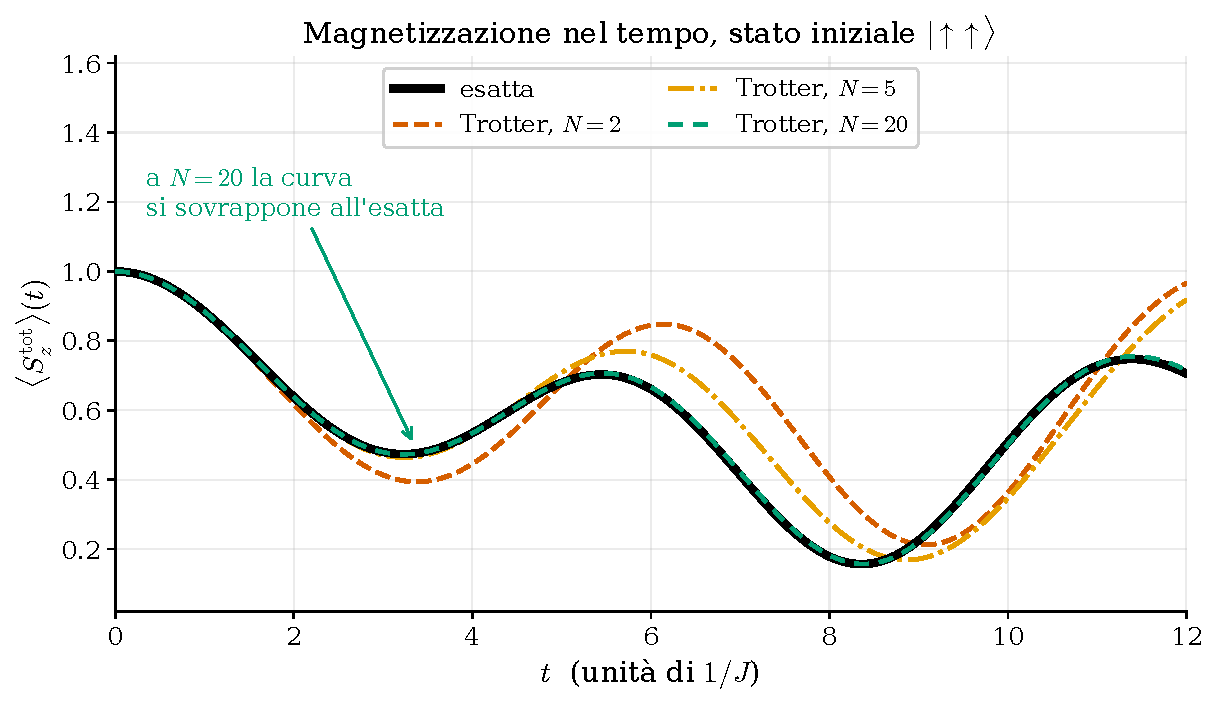
\includegraphics[width=0.86\textwidth]{figure/fig05_trotter_sz}
\caption{Magnetizzazione totale in funzione del tempo. La curva nera è
l'evoluzione esatta. Con soli $2$ passi (rosso) il circuito sbaglia visibilmente
ampiezza e fase; con $5$ passi (arancio) l'errore si riduce ma resta; con $20$
passi (verde) la curva si sovrappone all'esatta e non è più distinguibile a
occhio. Il punto di lavoro è scelto perché la dinamica non sia monocromatica:
un'unica frequenza renderebbe l'errore molto più difficile da vedere.}
\label{fig:sz}
\end{figure}

\FloatBarrier

\needspace{9\baselineskip}
\section{L'errore si comporta come previsto}

L'affermazione ``l'errore va come $1/N$'' è verificabile, e va verificata: è il
modo di distinguere un'approssimazione controllata da un'approssimazione che si
spera vada bene.

La prima colonna della tabella e della figura che seguono ($\lVert
U_{\rm Trotter}-U_{\rm esatto}\rVert$) misura quanto differiscono, nel caso
peggiore, i due operatori di evoluzione --- non punto per punto, ma come
oggetti nel loro complesso: quanto possono al massimo allontanarsi due stati
fatti evolvere l'uno con $U_{\rm Trotter}$ e l'altro con $U_{\rm esatto}$,
qualunque sia lo stato di partenza. È un numero più severo della sola
differenza sullo stato che stiamo davvero usando (colonna centrale): tiene
conto anche degli stati che non abbiamo provato.

\begin{figure}[htbp]
\centering
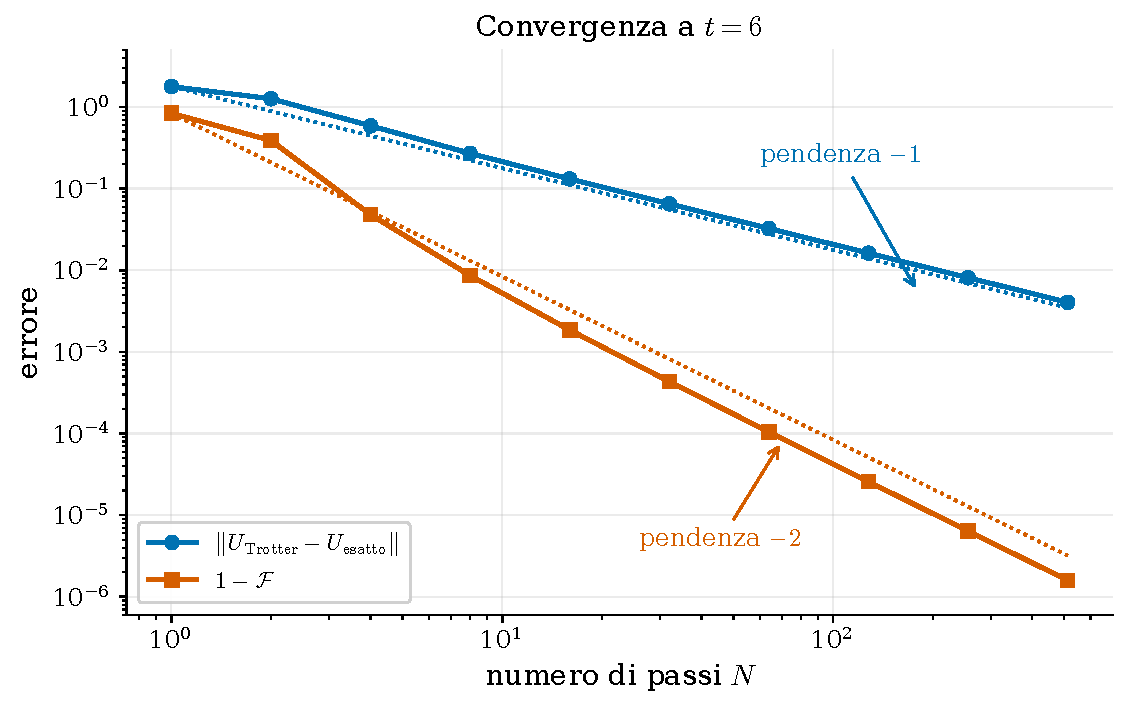
\includegraphics[width=0.76\textwidth]{figure/fig06_trotter_errore}
\caption{Errore a tempo fissato ($t=6$) al crescere del numero di passi, in
scala doppio-logaritmica. Le due grandezze misurano cose diverse: la distanza
fra gli operatori di evoluzione (blu) scala come $1/N$, la perdita di fidelity
sullo stato (rosso) come $1/N^2$. Le rette punteggiate sono le pendenze attese,
ancorate al primo punto. Gli scostamenti a $N$ piccolo sono i termini di ordine
superiore, che a pochi passi non sono trascurabili.}
\label{fig:errore}
\end{figure}

\FloatBarrier

\begin{table}[htbp]
\centering
\small
\renewcommand{\arraystretch}{1.25}
\begin{tabular}{@{}rccc@{}}
\toprule
\rowcolor{grigetto}
$N$ & $\lVert U_{\rm Trotter}-U_{\rm esatto}\rVert$ & $1-\mathcal F$ & $\lvert\Delta\media{S_z}\rvert$ \\
\midrule
  2 & $1.26$ & $3.9\times10^{-1}$ & $1.8\times10^{-1}$ \\
  8 & $2.7\times10^{-1}$ & $8.6\times10^{-3}$ & $3.8\times10^{-2}$ \\
 32 & $6.5\times10^{-2}$ & $4.3\times10^{-4}$ & $2.3\times10^{-3}$ \\
128 & $1.6\times10^{-2}$ & $2.6\times10^{-5}$ & $1.5\times10^{-4}$ \\
512 & $4.0\times10^{-3}$ & $1.6\times10^{-6}$ & $9.1\times10^{-6}$ \\
\bottomrule
\end{tabular}
\caption{Errore a $t=6$. Raddoppiando i passi, la prima colonna si dimezza e la
seconda si divide per quattro: è esattamente il comportamento atteso. Le
pendenze misurate con un fit sui punti con $N\ge8$ valgono $-1.008$ e $-2.059$
contro i valori teorici $-1$ e $-2$.}
\end{table}

\FloatBarrier

\needspace{9\baselineskip}
\section{Quanto costa: la parte che decide se è fattibile su hardware}

Il numero di passi non è gratis. Ogni passo aggiunge porte, e sull'hardware
reale sono le porte a due qubit a dominare il tasso di errore. Contarle è quindi
la misura di fattibilità più diretta.

Un chiarimento prima della tabella, perché il conteggio che segue non si legge
a occhio dalla Fig.~\ref{fig:circ-trotter}: il circuito \emph{come disegnato} usa $5$
porte a due qubit per passo ($R_{xx}$, $R_{yy}$ e tre $R_{zz}$ --- una per lo
scambio, due coniugate da Hadamard per il DM), scelte apposta perché ciascuna
corrisponda a un pezzo fisico riconoscibile dell'Hamiltoniana. La tabella,
invece, conta le porte \emph{dopo aver ricompilato da capo} l'intero passo su
un set hardware realistico (CNOT più rotazioni a un qubit): il compilatore non
traduce le $5$ porte una per una, riconosce che insieme realizzano un unico
operatore unitario a due qubit e lo risintetizza con la decomposizione ottima
nota per un gate a due qubit arbitrario (al più $3$ CNOT, un risultato
classico). Sono due circuiti diversi --- uno leggibile, l'altro minimo --- non
lo stesso circuito contato in due modi.

\begin{table}[htbp]
\centering
\small
\renewcommand{\arraystretch}{1.3}
\begin{tabular}{@{}lcc@{}}
\toprule
\rowcolor{grigetto}
\textbf{Compilazione} & \textbf{CNOT per passo} & \textbf{profondità} \\
\midrule
traduzione diretta, nessuna ottimizzazione & $10$ & $37$ \\
compilazione ottimizzata & $\mathbf{3}$ & $13$ \\
\bottomrule
\end{tabular}
\caption{Costo di un passo di Trotter, contato dopo la traduzione nel set di
porte nativo. Chiedere al compilatore di minimizzare riduce le porte a due
qubit di un fattore superiore a tre. Non è una raffinatezza: su hardware reale
il numero di CNOT è il fattore che determina quanto lontano si può spingere
l'evoluzione prima che il rumore la distrugga.}
\end{table}

\FloatBarrier

\messaggio{C'è una tensione strutturale fra i due risultati di questo documento:
l'errore di Trotter scende aumentando $N$, ma l'errore hardware sale, perché il
circuito si allunga di $3$ CNOT per ogni passo aggiunto. Esiste quindi un $N$
ottimo, e non è né il più piccolo né il più grande. Determinarlo richiede un
modello di rumore: è il ponte naturale verso quando studieremo il sistema
come sistema aperto.}

\section{Nota sul punto di lavoro}

Le figure~\ref{fig:sz} e~\ref{fig:errore} usano $b/J=-0.18$, $D/J=1$, con stato
iniziale $\ket{\uparrow\uparrow}$. La scelta è deliberata e vale la pena
motivarla, perché è un punto metodologico che si ripresenta: uno stato iniziale
che sia già autostato dei singoli blocchi dell'Hamiltoniana evolve in modo
banale e \emph{non mostra} l'errore di Trotter, anche quando c'è. Un test di
convergenza fatto su uno stato del genere darebbe un risultato ottimo e privo di
significato. Servono uno stato e un punto di lavoro asimmetrici, che facciano
emergere l'errore invece di mascherarlo.

\needspace{9\baselineskip}
\section{Quando anche lo stato di partenza è imperfetto}

$\ket{\uparrow\uparrow}$ è comodo perché è autosufficiente: non richiede nulla
da nessun altro documento. Ma il Documento 2 ha già costruito due stati di
partenza veri e propri --- quelli prodotti dal VQE --- e a questo stesso punto
di lavoro le loro fidelity sono molto diverse fra loro (vedi la tabella di
confronto nel Documento 2, \S6): $0.9229$ per l'ansatz minimo,
$1$ (a dodici cifre) per quello esteso. È l'occasione per chiedersi cosa
succede quando i due errori del progetto --- quello di preparazione e quello
di evoluzione --- agiscono insieme, e se un ansatz migliore basta a farlo
sparire.

\begin{figure}[htbp]
\centering
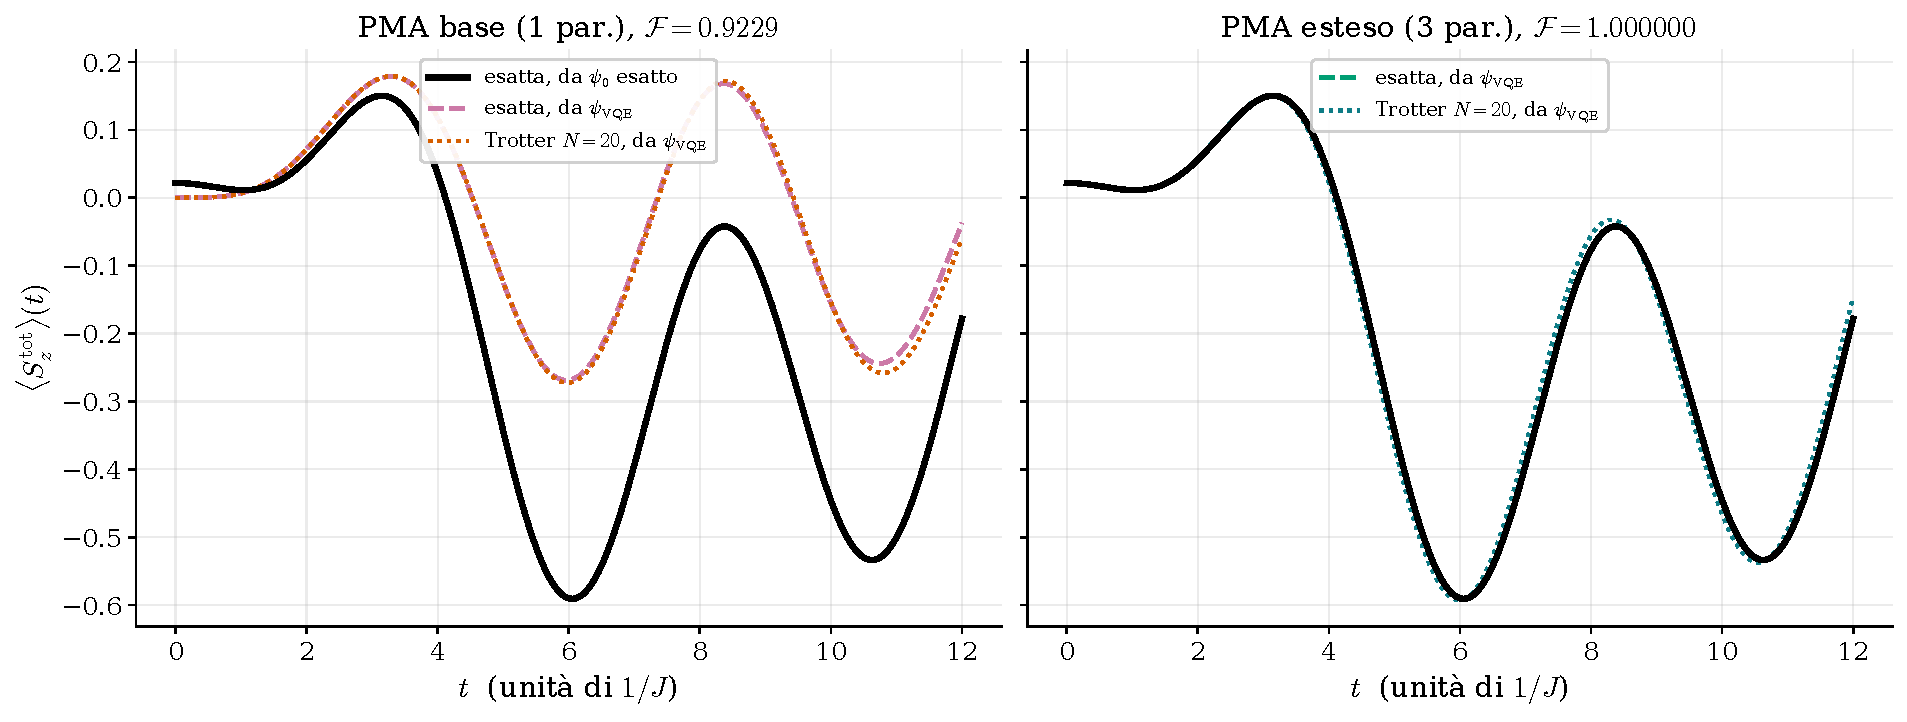
\includegraphics[width=\textwidth]{figure/fig12_trotter_due_ansatz}
\caption{Stesso punto di lavoro, stesso trattamento, due ansatz diversi dal
Documento 2. In entrambi i pannelli: nera, l'evoluzione esatta dal
fondamentale esatto (il riferimento); tratteggiata, evoluzione \emph{esatta}
ma a partire dallo stato del VQE (isola l'errore di preparazione); punteggiata,
evoluzione di \emph{Trotter} ($N=20$) dallo stesso stato del VQE (entrambi gli
errori insieme). \textbf{A sinistra}, PMA base: le due curve del VQE si
staccano nettamente da quella esatta. \textbf{A destra}, PMA esteso: tutte e
tre le curve sono indistinguibili a occhio.}
\label{fig:trotter-vqe}
\end{figure}

\FloatBarrier

I numeri confermano quello che si vede, per entrambi gli ansatz:

\begin{table}[htbp]
\centering
\small
\renewcommand{\arraystretch}{1.3}
\begin{tabular}{@{}lccc@{}}
\toprule
\rowcolor{grigetto}
\textbf{ansatz} & \textbf{solo VQE} & \textbf{VQE + Trotter} & \textbf{solo Trotter (da VQE)} \\
\midrule
PMA base (1 par.) & $0.327$ & $0.322$ & $0.024$ \\
PMA esteso (3 par.) & $0.000$ & $0.033$ & $0.033$ \\
\bottomrule
\end{tabular}
\caption{Scarto massimo su $\langle S_z^{\rm tot}\rangle(t)$, scomposto come
in Fig.~\ref{fig:trotter-vqe}. Con l'ansatz minimo l'errore di preparazione
($0.327$) domina quello di Trotter di più di dieci volte. Con l'ansatz esteso
l'errore di preparazione sparisce del tutto (per costruzione: $\mathcal
F\approx1$), e quello che resta --- $0.033$ --- è \emph{solo} Trotter: non
identico all'errore puro già misurato in Fig.~\ref{fig:sz} da
$\ket{\uparrow\uparrow}$ allo stesso $N$ (che vale $0.010$ sullo stesso
intervallo) --- stati diversi hanno contenuto in frequenza diverso, quindi
anche il loro errore di Trotter differisce --- ma dello stesso ordine di
grandezza, e comunque molto più piccolo dell'errore di preparazione
dell'ansatz minimo.}
\label{tab:doppio-errore}
\end{table}

\FloatBarrier

Con $N=20$, in questo punto, l'ansatz minimo lascia sul tavolo un errore di
preparazione dieci volte più grande di quello di Trotter: aumentare $N$ non
lo tocca nemmeno. Con l'ansatz esteso quell'errore sparisce, e resta solo
quello che aumentare $N$ può davvero ridurre.

\messaggio{I due errori del progetto non sono intercambiabili, e la Tab.~
\ref{tab:doppio-errore} lo misura invece di limitarsi ad affermarlo: qui
aumentare $N$ oltre un certo punto non migliorerebbe quasi nulla finché lo
stato di partenza resta quello del PMA base. Tornare al Documento 2 e usare
l'ansatz esteso elimina un errore dieci volte più grande di quello che
Trotter lascia --- prima di spendere altri CNOT in altri passi.}

\bigskip
\noindent\footnotesize\textit{Riferimento.} Per la norma usata a confrontare
gli operatori di evoluzione (il più grande fattore di allungamento che la
matrice può applicare a un vettore): R.~A.~Horn, C.~R.~Johnson, \emph{Matrix
Analysis}, Cambridge University Press, 2ª ed.\ (2012), cap.~5.

\end{document}
